\documentclass{ximera}

%\addPrintStyle{..}


\begin{document}
	\author{Bart Lambregs}
	\xmtitle{Oefeningen tweedimensionale bewegingen}{}
    \xmsource\xmuitleg

% VRAAGSTUK VAN FYSICA VANDAAG = VERVANGEN DOOR IETS ANDERS?
% % 2d_I_1 % FV 14 p. 88
% \begin{exercise}

% % 14 p. 88
%  Twee duikers duiken horizontaal van een duikplatform. De bovenste duiker A start tweemaal hoger boven het water dan de onderste duiker. De horizontale beginsnelheid van de onderste duiker is tweemaal zo groot als die van de bovenste. De duikers komen terecht in het water op horizontale afstanden $x_a$ en $x_b$ van de plank. Wat is de verhouding van de horizontale afstanden?
% %\newline
% %\newline
% %\begin{tabularx}{\textwidth}{XXXX}
% %(a) $\displaystyle\frac{x_a}{x_b}=\frac{1}{\sqrt{2}}$&(b) $\displaystyle\frac{x_a}{x_b}=1$&(c) $\displaystyle\frac{x_a}{x_b}=\sqrt{2}$&(d) $\displaystyle\frac{x_a}{x_b}=2$
% %\end{tabularx}
% %
% %\begin{figure}[H]
% %\centering
% %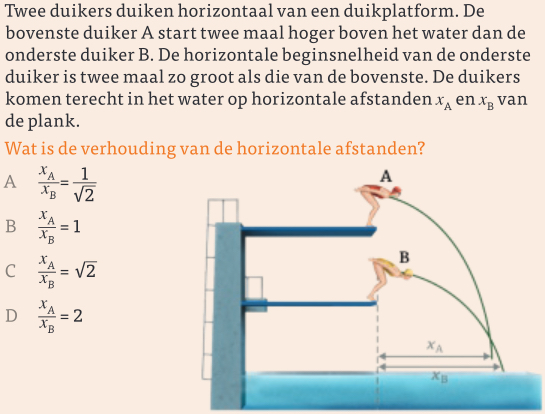
\includegraphics[width=0.6\textwidth]{dyn/exercises/14p88}
% %\end{figure}
% \begin{minipage}[t]{.3\textwidth}
% \begin{enumerate}
% \item $\displaystyle\frac{x_a}{x_b}=\frac{1}{\sqrt{2}}$
% \item $\displaystyle\frac{x_a}{x_b}=1$
% \item $\displaystyle\frac{x_a}{x_b}=\sqrt{2}$
% \item $\displaystyle\frac{x_a}{x_b}=2$
% \end{enumerate}
% \end{minipage}
% \hfill
% \begin{minipage}[t]{.5\textwidth}
% 	\raisebox{1ex-\height}{%
% 		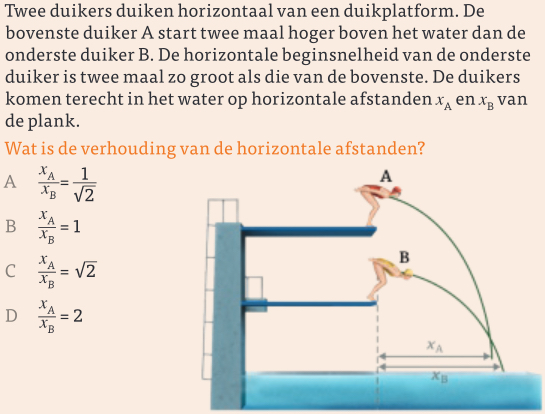
\includegraphics[width=\textwidth]{dyn/exercises/14p88}} 
% \end{minipage}
% \begin{oplossing}
% % \newline
% In verticale zin hebben beide duikers geen beginsnelheid en versnellen ze met de valversnelling. In verticale zin voeren ze dus een EVRB uit. De valtijd vind je dan uit $y=\frac{1}{2}gt^2$, nl. $t=\sqrt{\frac{2y}{g}}$.

% In horizontale zin hebben de duikers geen versnelling en houden dus (volgens de wet van de traagheid) hun initi\"ele snelheid aan. De afgelegde weg volgens de horizontale $x$-as vinden we dan ook met $x=v_0t$ waarin $v_0$ de (horizontale) beginsnelheid is en waarin we $t$ door de valtijd kunnen vervangen.

% Gebruik nu dat $y_a=2y_b$ en $v_{0b}=2v_{0a}$ en bereken de gevraagde verhouding.
% \end{oplossing}

% \end{exercise}




% VRAAGSTUK VAN FYSICA VANDAAG = VERVANGEN DOOR IETS ANDERS?

% % 2d_I_2 % FV 6 p. 92 
% \begin{exercise}

% % !TEX root = ../main.tex



% [6 p. 92]  
% \begin{minipage}[t]{.5\textwidth}
% Een bal K gooi je vooruit en een bal L gooi je tegelijk naar beneden. Ze komen tegelijk aan in M. Met welke snelheid heb je bal L gegooid?
% \end{minipage}
% \hfill
% \begin{minipage}[t]{.4\textwidth}
% 	\raisebox{1ex-\height}{%
% 		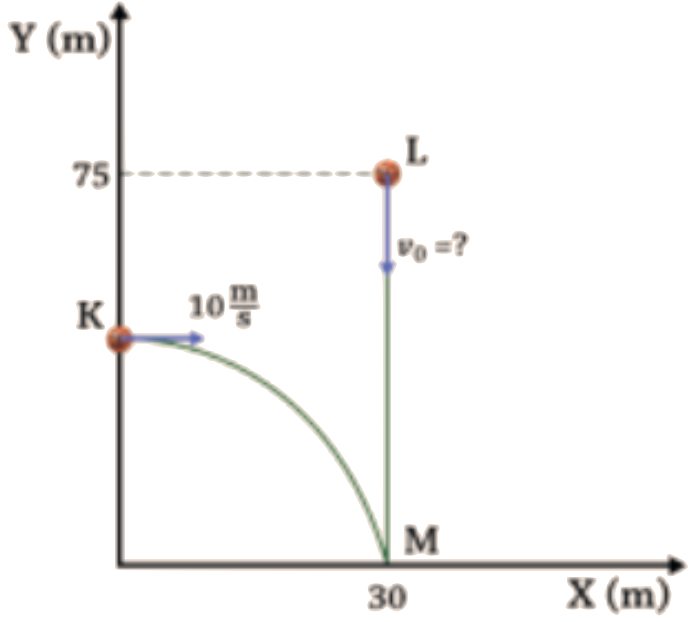
\includegraphics[width=\textwidth]{dyn/exercises/6p92}} 
% \end{minipage}
% \begin{oplossing}
% % \newline
% In horizontale zin voert bal K een ERB uit. Hij heeft dan ook 3 seconden nodig om M te bereiken. Die tijd is ook de valtijd voor L en kunnen we gebruiken om $v_0$ in verticale zin te bepalen. Uit $0=y_0+v_0t-\frac{1}{2}gt^2$ (de as staat omhoog gericht) vinden we 
% \begin{eqnarray*}
% v_0&=&\frac{\frac{1}{2}gt^2-y_0}{t}
% \end{eqnarray*}
% of $v_0=\SI{-10,29}{m/s}$. Merk op dat die beginsnelheid negatief is. De zin is tegengesteld aan de omhoog gerichte $y$-as.
% \end{oplossing}

% \end{exercise}




% VANAF HIER BART_E2DIM_NOIMPORT.TEX 

% DERGELIJKE theorieVRAGEN HIER NIET STELLEN?
% \begin{exercise} Toon aan dat de versnelling bij een ECB een middelpuntzoekende versnelling is.
% \end{exercise}

% DERGELIJKE VRAGEN HIER NIET STELLEN?
% \begin{exercise} Voor een ECB heb je bewezen dat de versnelling wordt gegeven door de formule $\vec{a}=-\omega^2\cdot\vec{r}$, met $\omega$ de hoeksnelheid en $\vec{r}$ de plaatsvector van de ECB. 

% Hoe kan je uit deze formule besluiten dat de versnelling bij een ECB een middelpuntzoekende versnelling is?
% \end{exercise}

% \begin{exercise}

% \begin{enumerate}
% \item \label{ECB_formule} Bewijs dat de versnelling van een ECB gegeven wordt door $\vec{a}=-\omega^2\cdot\vec{r}$. Hierin is $\omega$ de hoeksnelheid en $\vec{r}$ de plaatsvector van de ECB.
% \item Hoe kan je uit de formule voor de versnelling in besluiten dat de versnelling bij een ECB een middelpuntzoekende versnelling is? % hier stond ref ECB label 
% \end{enumerate}

% \begin{oplossing}
% Voor (a):
% \begin{enumerate}
% \item[1p] Kiezen assenstelsel met oorsprong in middelpunt van de cirkel
% \item[1p] $\vec{r}=$
% \item[1p] $\frac{d^2 \vec{r}}{dt^2}=$
% \item[1p] $=-\omega^2\cdot\vec{r} $
% \item[1p] Uitleg/kadering, niet enkel opeenvolging van formules
% \end{enumerate}
% Voor (b) twee punten, voor argument voor de zin en argument voor de richting
% \end{oplossing}

% \end{exercise}

% \begin{exercise} Bewijs dat de snelheid aan de baan raakt.
% \end{exercise}

\begin{exercise}
	Welk punt heeft de grootste versnelling: een punt op de buitenrand van een ronddraaiende cd, of een punt op de helft van de straal van een cd die met een tweemaal zo grote hoeksnelheid ronddraait? Toon je antwoord aan.
\end{exercise}

\begin{exercise}
	Een bal wordt in een horizontale richting van de rand van een rotswand gegooid, met beginsnelheid $v_0$. De hoek die de bewegingsrichting van de bal op een willekeurig moment met de horizontaal maakt, noemen we $\theta$. Leid een formule af die voor de periode dat de bal onderweg is de hoek $\theta$ als functie van $t$ geeft.
\end{exercise}

\begin{exercise}
	Een tennisspeler, die \SI{9,0}{\meter} voor het net staat, slaat een bal in horizontale richting met een snelheid van \SI{25}{\meter\per\second}. Het racket raakt de bal \SI{1,8}{\meter} boven de grond. De bovenkant van het net is \SI{1,0}{\meter} boven de grond. Vliegt de bal over het net, of er tegenaan?
\end{exercise}

\begin{exercise}
	Een pijl, die horizontaal wordt afgeschoten in het punt $P$ treft een verticale wand in punt (1). Verdubbelt men de vertreksnelheid van de pijl in het punt P, dan zal de pijl dezelfde wand treffen:
	\newline

	\begin{minipage}{0.4\textwidth}
		\begin{multipleChoice}
			\choice{in het punt (1)}
			\choice{in het punt (2)}
			\choice[correct]{in het punt (3)}
			\choice{in het punt (4)}
		\end{multipleChoice}
	\end{minipage}
	\hfill
	\begin{minipage}{0.6\textwidth}
		\begin{image}
			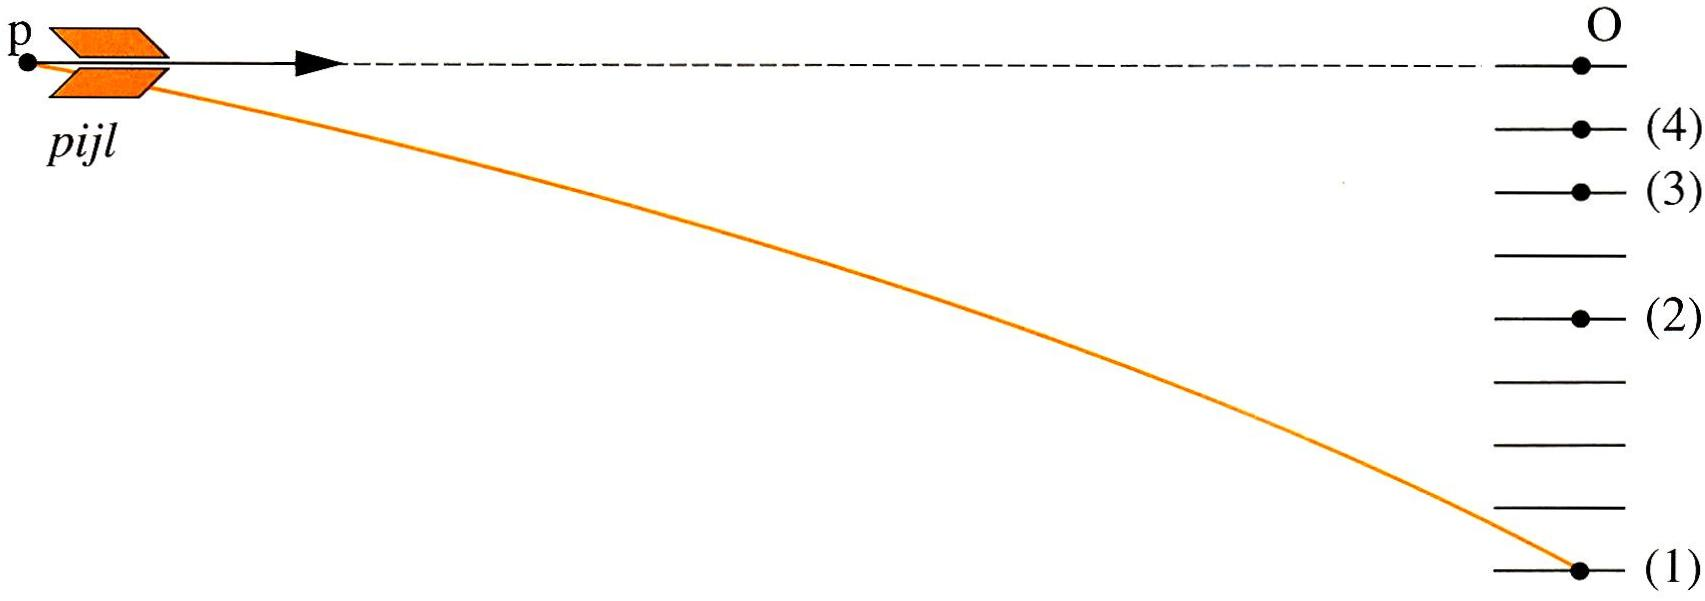
\includegraphics{afgeschotenpijl}
		\end{image}
	\end{minipage}

\begin{oplossing}
	We gebruiken de baanvergelijking van de horizontale worp. Voor eenzelfde horizontale afstand $x$ moeten we immers een nieuwe verticale afstand $y$ vinden, in functie van een andere beginsnelheid. Als het accent ' staat voor de nieuwe situatie waarin de beginsnelheid is verdubbeld, dan geldt:
	\begin{eqnarray*}
		y'&=&\frac{g}{2v_0'^2}x^2\\
		&=&\frac{g}{2(2v_0)^2}x^2\\
		&=&\frac{1}{4}\frac{g}{2v_0^2}x^2\\
		&=&\frac{1}{4}y
	\end{eqnarray*}
	De pijl zal dus in punt (3) terechtkomen.
\end{oplossing}
\end{exercise}

\begin{exercise}
	Een puntmassa beschrijft een cirkel met een straal van\SI{5,0}{\centi\meter} en een periode van \SI{0,33}{\second}. Welke afstand op de cirkel legt deze puntmassa in \SI{7,0}{\second} af?
	\begin{oplossing}
		Omdat de grootte van de snelheid constant is, is de
		afgelegde weg over de boog gelijk aan de snelheid vermenigvuldigd met de tijd:
		\begin{eqnarray*}
			s&=&vt\\
			&=&r\omega t\\
			&=&\frac{2\pi r}{T}t\\
			&=&6,7\rm\,m
		\end{eqnarray*}
	\end{oplossing}
\end{exercise}

\begin{exercise}
	Bereken de hoeksnelheid van de aarde om haar as. Bereken de snelheid van een punt van het aardoppervlak:
	\begin{enumerate}
		\item aan de evenaar,
		\item op $\SI{51}{\degree}$ noorderbreedte.
	\end{enumerate}
	\begin{oplossing}
		De hoeksnelheid kunnen we berekenen met de periode van de omwenteling van de aarde, nl. 24 uur, t.t.z. \SI{86400}{\second}. Dat geeft
		\begin{eqnarray*}
			\omega=\frac{2\pi}{T}=\frac{2\pi}{\SI{86400}{\second}}=\SI{7,3e-5}{\radian\per\second}
		\end{eqnarray*}
		De snelheid van een punt op het aardoppervlak aan de evenaar vinden we met het formuletje $v=r\omega$, waarbij $r$ de straal van de aarde\footnote{De straal van de aarde bedraagt \SI{6370}{\kilo\meter}.} is.
		\begin{eqnarray*}
		v=r_a\omega=\frac{2\pi r_a}{T}=\SI{463}{\meter\per\second}%463\rm\,m/s
		\end{eqnarray*}
		Dit is nogal snel, het is namelijk \SI{1667}{\kilo\meter\per\hour}.% $1667\rm\,km/h$.

		Op $\SI{51}{\degree}$ noorderbreedte\footnote{Onze school ligt op $50^\circ 52'36,\!69''$ noorderbreedte.} maken we ook een cirkelbeweging maar nu met een andere straal. De straal is nu de afstand van het punt op het aardoppervlak tot aan de rotatieas van de aarde, zie figuur. 
		\begin{image}
		% \centering
		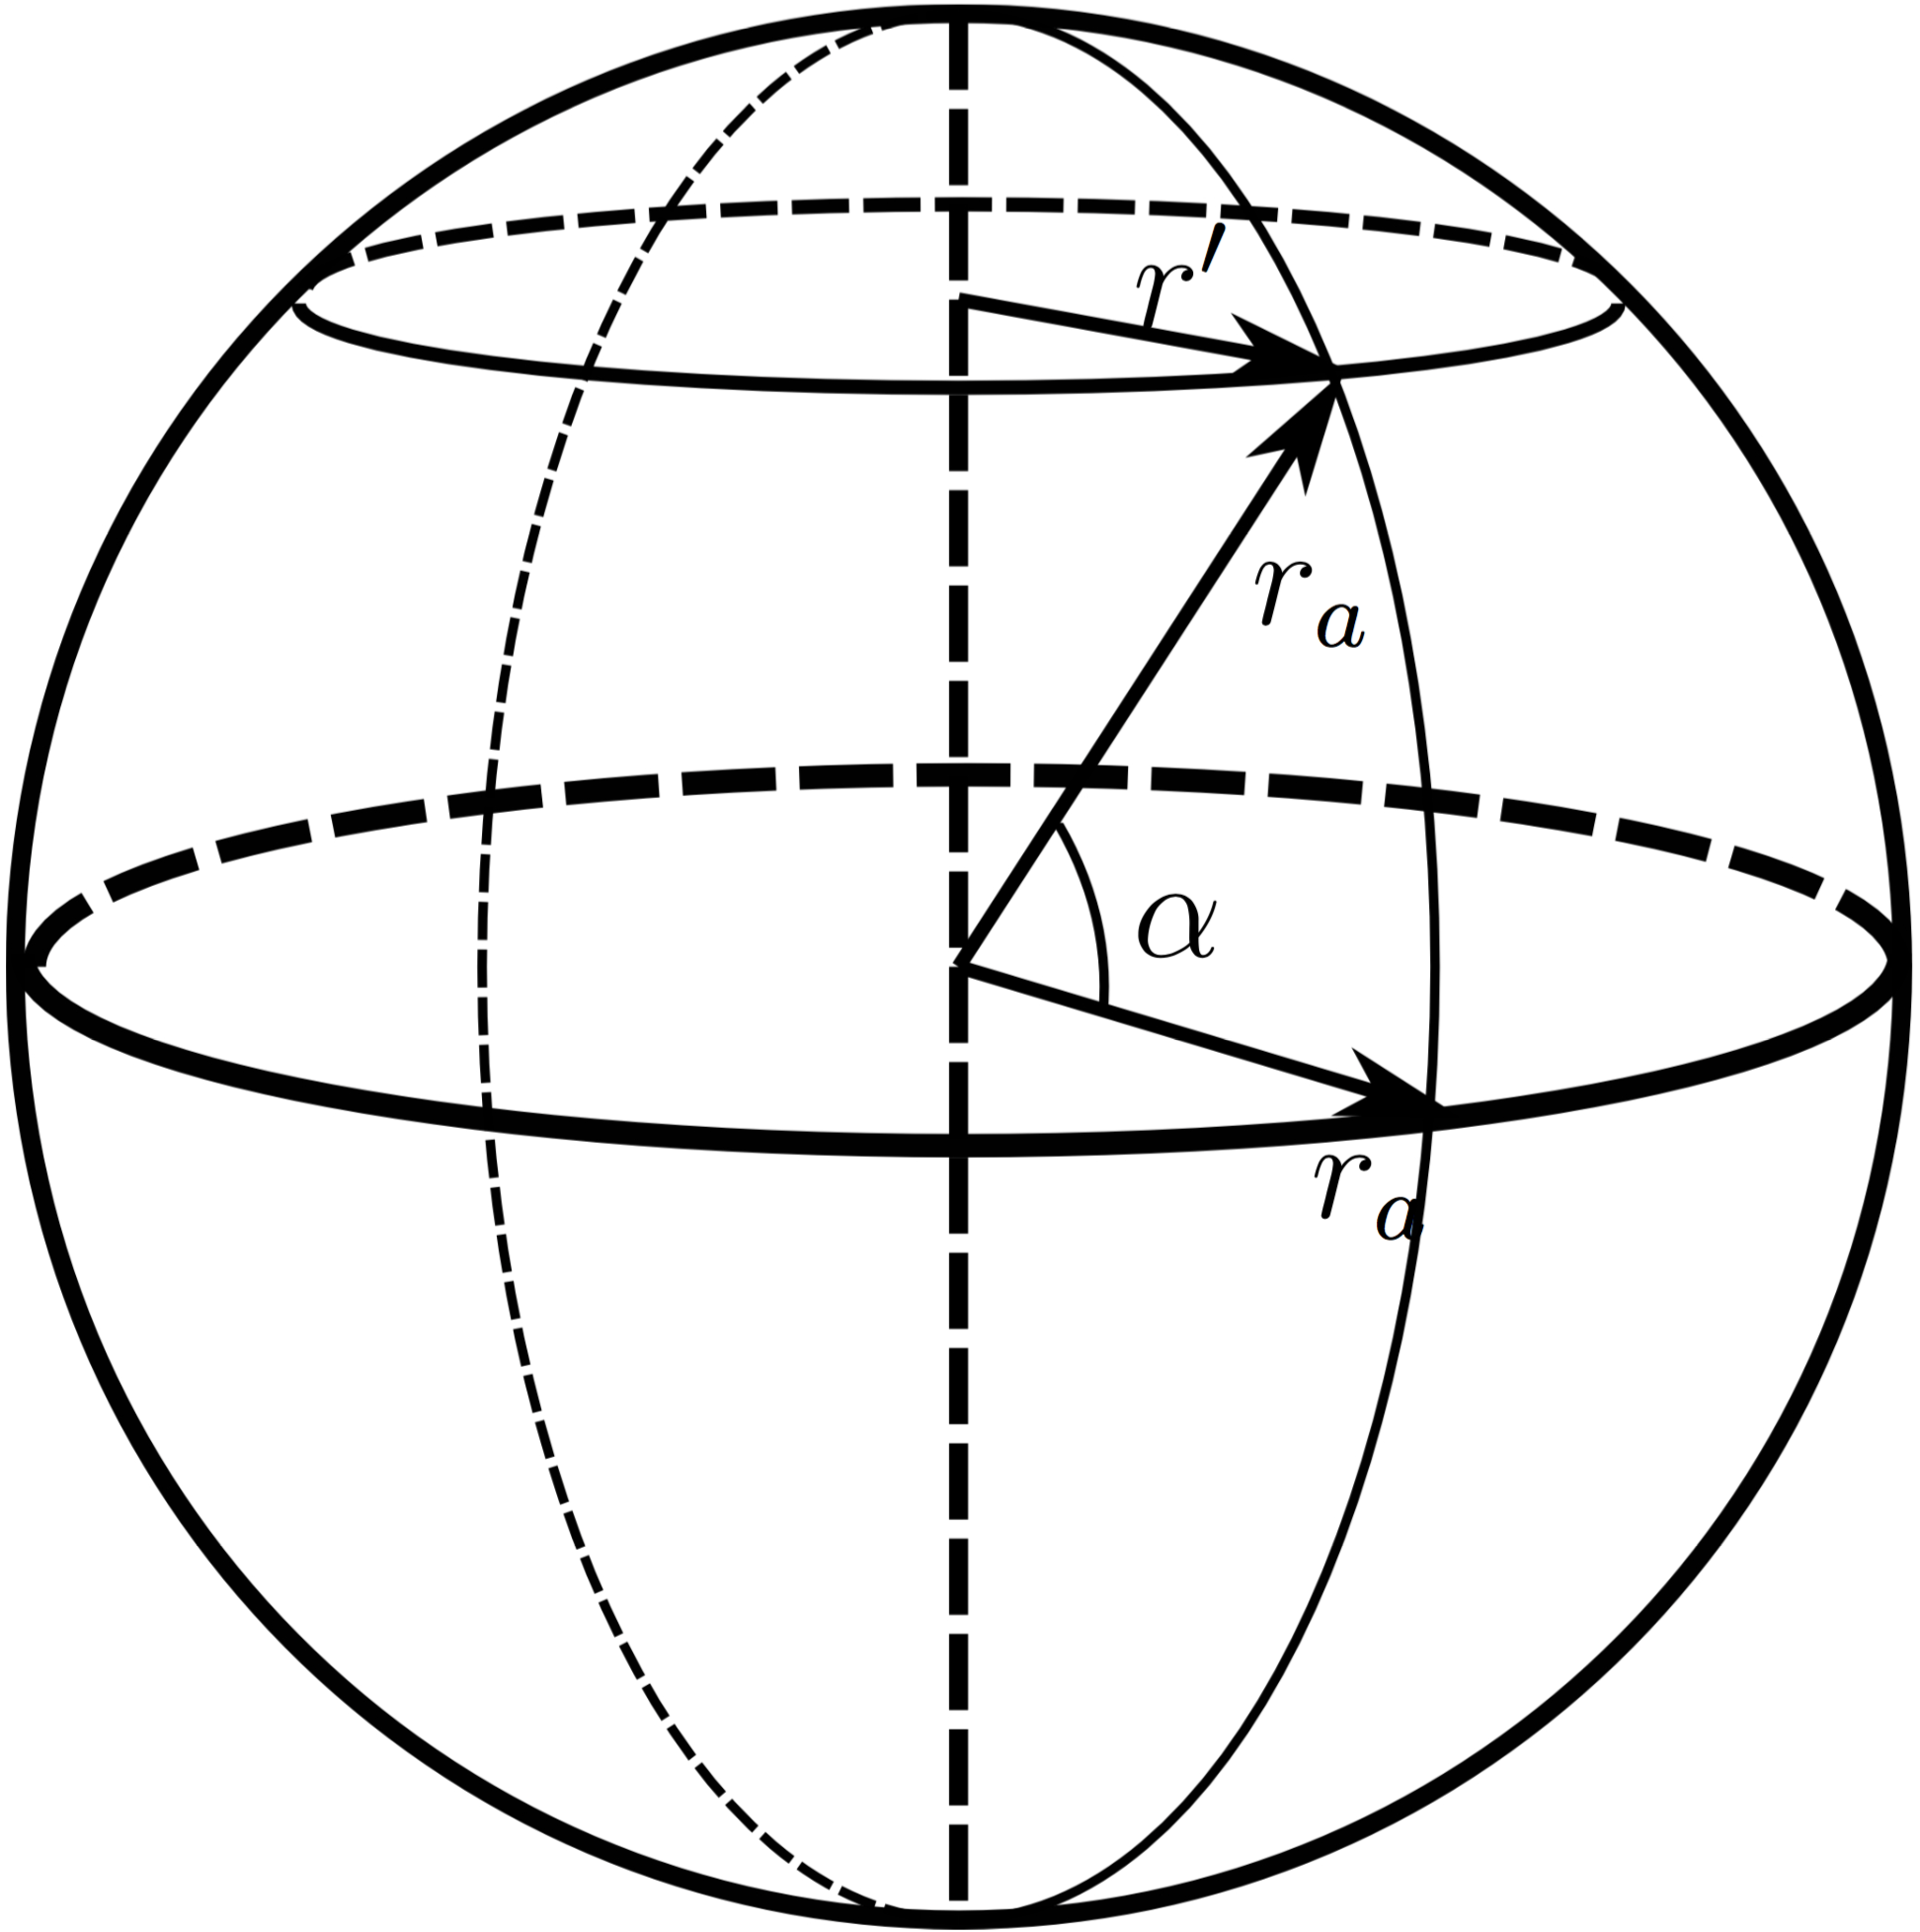
\includegraphics[width=0.4\textwidth]{aardehoeksnelheid2}
		\end{image}
		%%%\begin{figure}[H]
		%\begin{picture}(320,160)(0,0)
		%\put(115,0){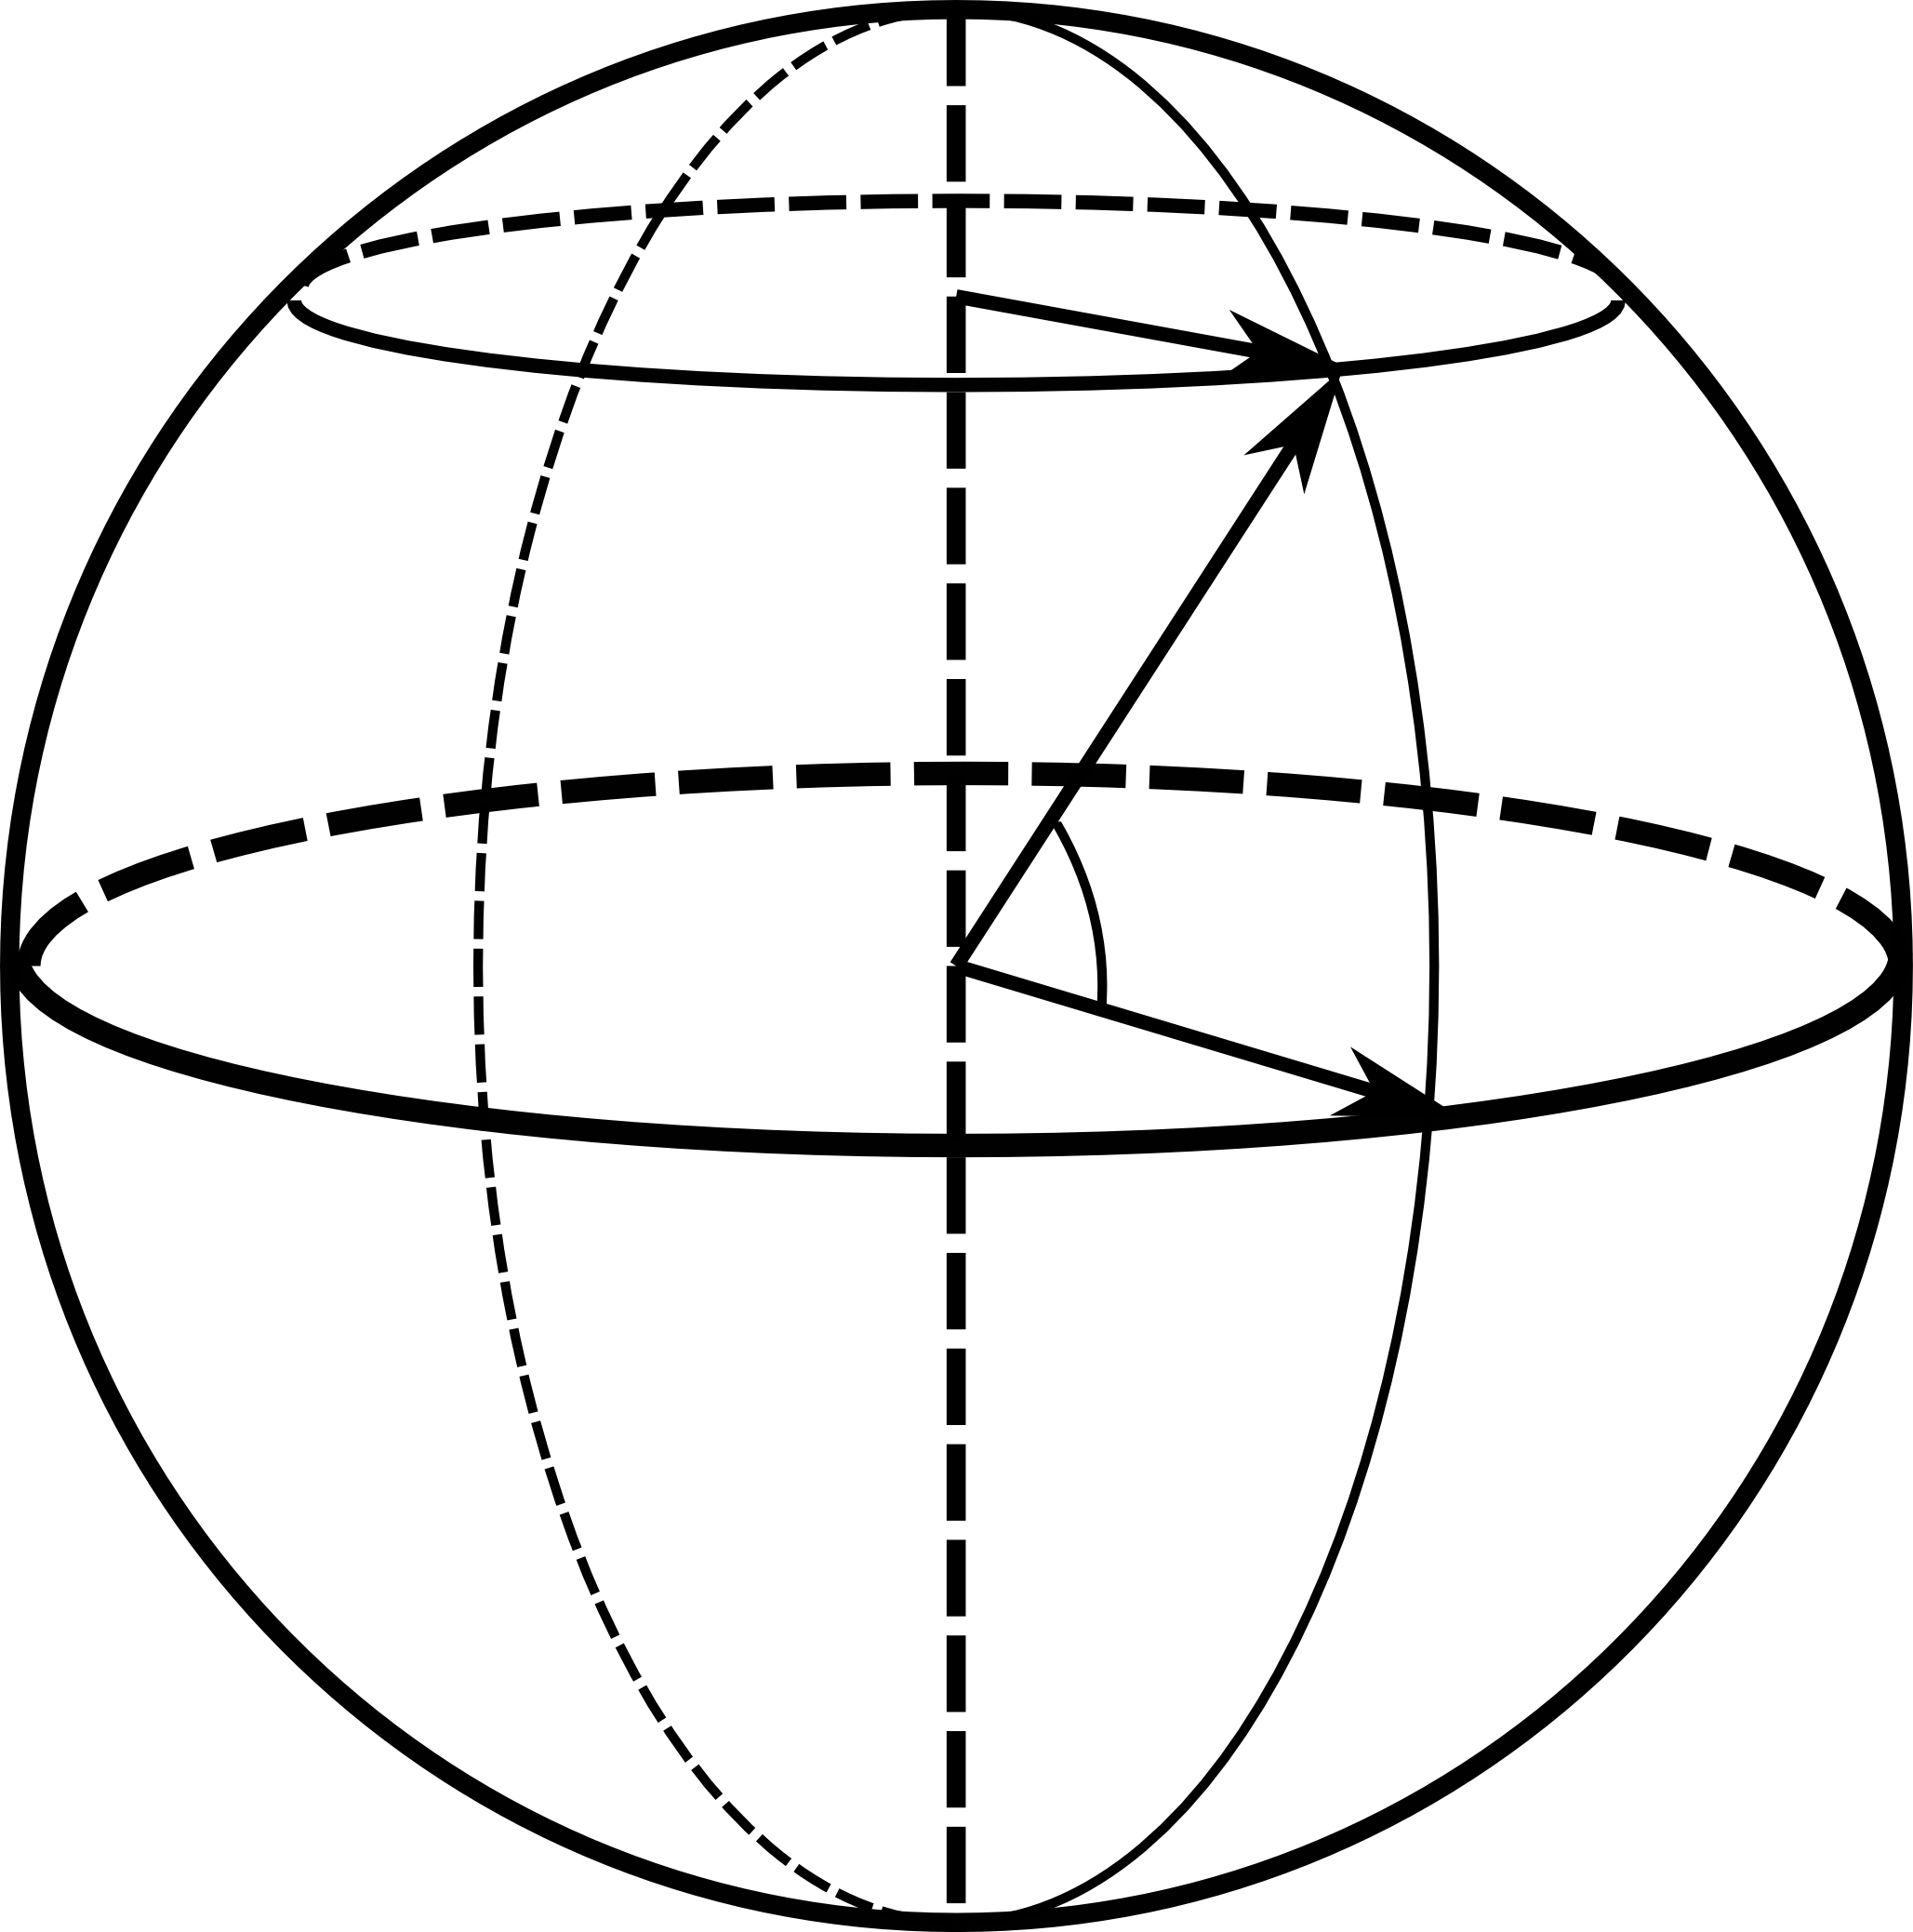
\includegraphics[scale=1.0]{aardehoeksnelheid}}
		%\put(210,82){$\alpha$}
		%\put(225,60){$r_a$}
		%\put(220,110){$r_a$}
		%\put(210,135){$r'$}
		%%\put(0,0){bl}
		%%\put(0,160){tl}
		%%\put(390,0){br}
		%%\put(390,160){.}
		%\end{picture}
		%%%\end{figure}
		Met elementaire driehoeksmeetkunde vind je deze straal terug als $r'=r\cos\alpha$. De snelheid vinden we vervolgens op dezelfde manier.
		\begin{eqnarray*}
		v=r'\omega=\frac{2\pi r\cos\alpha}{T}=\SI{291}{\meter\per\second}
		\end{eqnarray*}
		Dit is ook nog snel, nl. \SI{1048}{\kilo\meter\per\hour}.
	\end{oplossing}
\end{exercise}

\begin{exercise}
	Een auto rijdt door een bocht met een constante snelheid van \SI{50}{\kilo\meter\per\hour}. Heeft de auto een andere versnelling wanneer hij diezelfde bocht neemt met een constante snelheid van \SI{70}{\kilo\meter\per\hour}? Licht je antwoord toe.
\end{exercise}

\begin{exercise}
	Als een auto met \SI{60}{\kilo\meter\per\hour} een scherpe bocht neemt, en daarna met dezelfde snelheid een flauwe bocht, is de versnelling dan in beide gevallen gelijk? Leg uit.
\end{exercise}

\begin{exercise}
	Tijdens het trainen van een ruimtevaarder wordt deze in een cirkelvormige beweging gebracht met een zetel, die zich aan het uiteinde van een horizontale arm van \SI{5,00}{\meter} lengte bevindt. Indien hij versnellingen tot $10g$ kan verdragen, wat is dan de toegelaten maximale snelheid, en het maximale toegelaten toerental?
\end{exercise}

\begin{exercise}
	Alle punten van een ring voeren een eenparige cirkelbeweging uit. De grootte van de snelheid in punt $A$ is $v_a$ en in punt $B$, $v_b$. Dan is
	\newline

	\begin{minipage}{0.5\textwidth}
		\begin{multipleChoice}
			\choice{$v_ar_a=v_br_b$}
			\choice[correct]{$v_br_a=v_ar_b$}
			\choice{$v_av_b=r_ar_b$}
			\choice{$v_a=v_b$}
		\end{multipleChoice}
	\end{minipage}
	\hfill
	\begin{minipage}{0.5\textwidth}
		\begin{image}
			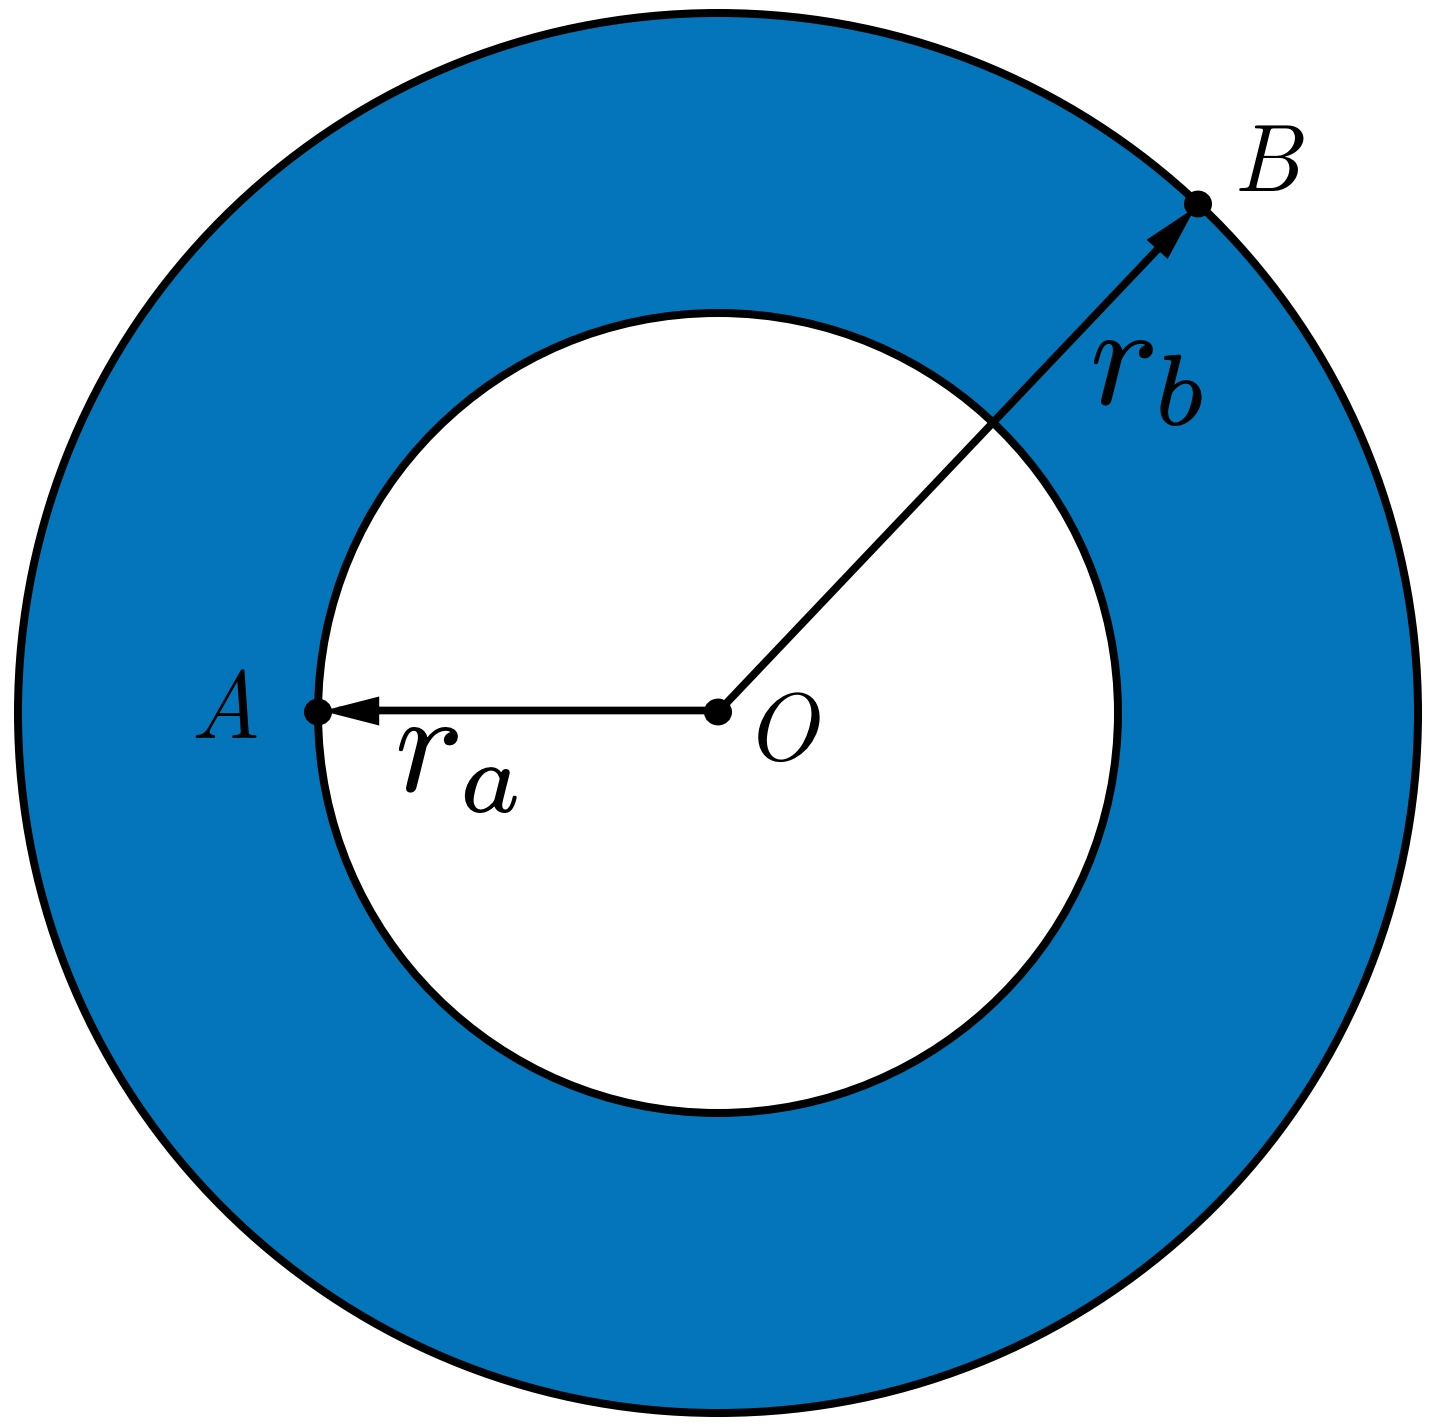
\includegraphics{ringpunten}
		\end{image}
	\end{minipage}

\begin{oplossing}
	De hoeksnelheid is voor beide punten gelijk zodat:
\begin{eqnarray*}
\omega_a&=&\omega_b\\
&\Updownarrow&\\
\frac{v_a}{r_a}&=&\frac{v_b}{r_b}\\
&\Updownarrow&\\
v_br_a&=&v_ar_b
\end{eqnarray*}
Het juist antwoord is dus (b).
\end{oplossing}
\end{exercise}

\begin{exercise}
	Bij een fiets zijn het grootste en het kleinste kamwiel door middel van een ketting met elkaar verbonden. Tussen de hoeksnelheid $\omega_1$ van het grootste kamwiel en $\omega_2$ van het kleinste kamwiel bestaat de volgende relatie:
	\newline

\begin{minipage}[t]{0.4\textwidth}
	\begin{multipleChoice}
		\choice{$\omega_1=\omega_2$}
		\choice{$r_1\omega_2=r_2\omega_1$}
		\choice[correct]{$r_1\omega_1=r_2\omega_2$}
		\choice{$r_1r_2=\omega_1\omega_2$}
	\end{multipleChoice}
\end{minipage}
\hfill
\begin{minipage}{0.5\textwidth}
		\begin{image}
			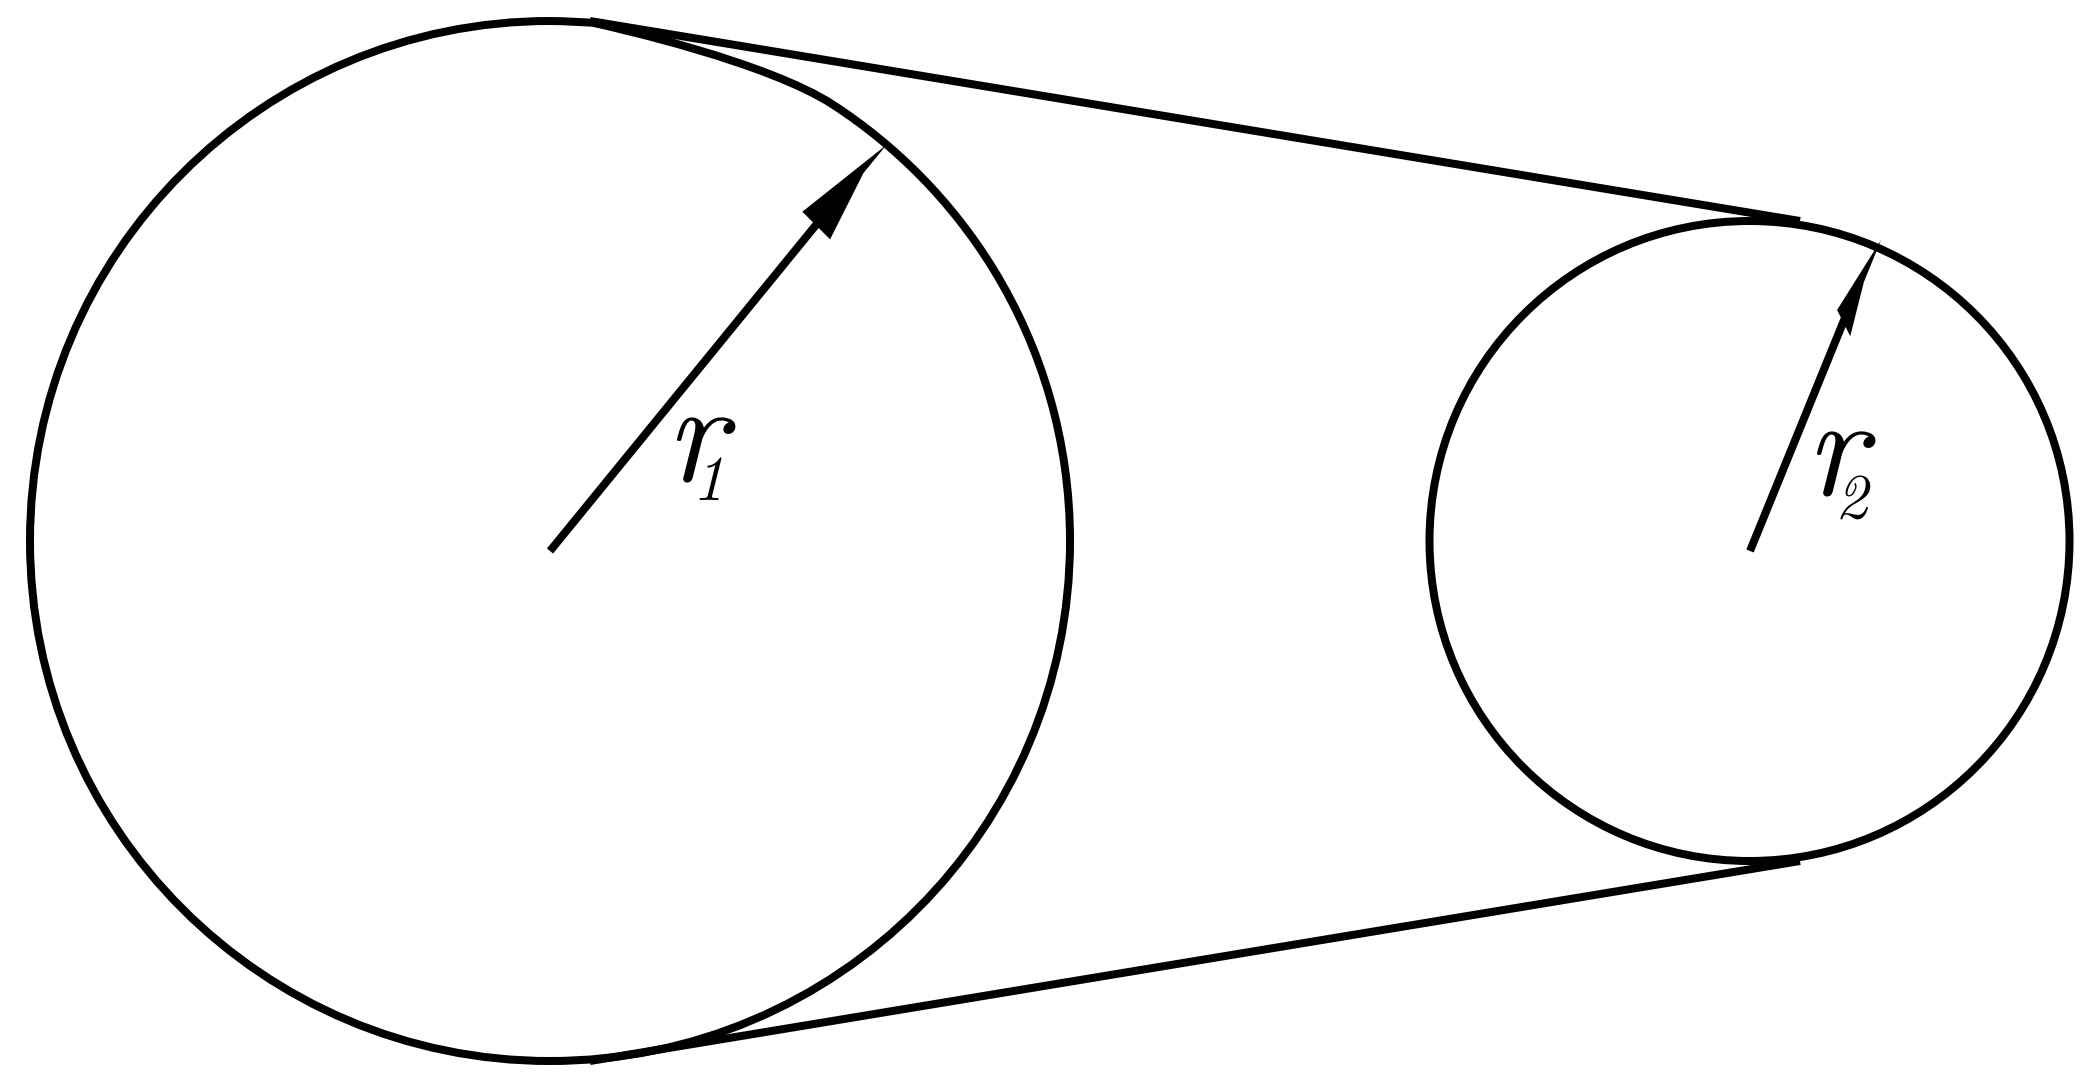
\includegraphics{kamwielenfiets}
		\end{image}
	\end{minipage}
\begin{oplossing}
	Aangezien een stukje van de ketting overal dezelfde snelheid heeft -- het legt in een bepaalde tijd steeds evenveel afstand af -- moet de snelheid van een punt op de buitenrand van het grootste wiel gelijk zijn aan de snelheid van een punt op de buitenrand van het kleinste wiel. Dus:
	\begin{eqnarray*}
		v_1&=&v_2\\
		&\Updownarrow&\\
		r_1\omega_1&=&r_2\omega_2
	\end{eqnarray*}
	Het juist antwoord is dus (c).
\end{oplossing}
\end{exercise}

\begin{exercise}
	Een auto rijdt door een brugleuning en komt \SI{5,2}{\meter} lager in het water terecht. De horizontale afstand tussen de plaats waar hij door de leuning ging en waar hij in het water terechtkwam, is \SI{22}{\meter}. Kan de politie hieruit afleiden met welke snelheid hij ongeveer reed? Was zijn werkelijke snelheid groter of kleiner?
	\begin{oplossing}
	\begin{eqnarray*}
		y&=&\frac{g}{2v_0^2}x^2\\
		&\Updownarrow&\\
		v_0&=&x\sqrt{\frac{g}{2y}}=21,37\rm\,m/s=\SI{77}{\kilo\meter\per\hour}
	\end{eqnarray*}
	\end{oplossing}
\end{exercise}

\begin{exercise}
	Een kogel wordt met een snelheid van \SI{800}{\meter\per\second} horizontaal afgeschoten op een doel dat zich op een horizontale afstand van \SI{100}{\meter} bevindt. Over welke afstand is de kogel afgezakt?
\end{exercise}

% Staat ook in de theorie
% \begin{exercise}
% 	Een vliegtuig vliegt met een snelheid van \SI{450}{\kilo\meter\per\hour} op een hoogte van \SI{920}{\meter}.
% 	\begin{enumerate}
% 		\item Hoe ver voor het doel moeten de voedselpakketten gelost worden om op het doel terecht te komen?
% 		\item Hoeveel tijd hebben de pakketten nodig om het doel te bereiken?
% 	\end{enumerate}
% 	\begin{oplossing}
% 		De afstand waarover de voedselpakketten in horizontale richting zijn vooruit gegaan, kunnen we vinden met de
% 		baanvergelijking. We weten namelijk hoever de pakketten naar beneden zijn gevallen en wat hun beginsnelheid is:
% 		\begin{eqnarray*}
% 			y&=&\frac{g}{2v_0^2}x^2\\
% 			&\Downarrow&\\
% 			x&=&v_0\sqrt{\frac{2y}{g}}=\SI{1712}{\meter}%1712\rm\,m
% 		\end{eqnarray*}
% 		De valtijd voor de pakketten vinden we o.a. door naar de verticale valbeweging te kijken. Deze gebeurt onafhankelijk van wat er in de horizontale richting gebeurt, zodat:
% 		\begin{eqnarray*}
% 			y&=&\frac{1}{2}gt^2\\
% 			&\Downarrow&\\
% 			t&=&\sqrt{\frac{2y}{g}}=\SI{13,7}{\second}%13,7\rm\,s
% 		\end{eqnarray*}
% 	\end{oplossing}
% \end{exercise}

\begin{exercise}
	Een vliegwiel doet 450 omwentelingen per minuut. Zoek de hoeksnelheid van het wiel en de snelheid van een punt op \SI{1,70}{\meter} van het middelpunt.
\end{exercise}

\begin{exercise}
	In een bocht met straal \SI{160}{\meter} verlaagt een autorenner zijn snelheid eenparig van \SI{90}{\meter\per\second} tot \SI{75}{\meter\per\second} in \SI{2}{\second}. Bereken de grootte van de versnelling van de wagen op het ogenblik dat de snelheid \SI{80}{\meter\per\second}.
\begin{multipleChoice}
\choice{\SI{40,7}{\meter\per\second\squared}}
\choice[correct]{\SI{40}{\meter\per\second\squared}}
\choice{\SI{15}{\meter\per\second\squared}}
\choice{\SI{7,5}{\meter\per\second\squared}}
\end{multipleChoice}
\end{exercise}

\begin{exercise} 
	In de figuur is de versnelling en de snelheid van een puntmassa gegeven op een bepaald tijdstip. De grootte van de versnelling is \SI{15,0}{\meter\per\second\squared} en de vector maakt een hoek van $\SI{30}{\degree}$ met de straal van de cirkel. De straal van de cirkel is \SI{2,50}{\meter}. Bepaal de grootte van de normaalversnelling, de grootte van de tangentiële versnelling en de grootte van de baansnelheid.
%ECB_tangentieel nog invoegen ... !
\end{exercise}





\end{document}
